\subsection{Problem Area}\label{sec:problemArea}
\comment{
Why are IoT Gateways so hard to get right? Why is the edge so hard to get right?
 - Diversity
 - Security
 - Stability
}

The space between the cloud and IoT and mobile devices, can be confusing at times. Knowing the history of IoT and the cloud is vital to understand the current developments. This, the methodology and the delimitation of this thesis will be discussed in the reminder of this section.\\
The terms used in the academic world and the industry are often different and many concepts partially overlap and complement each other making it hard to clearly categorize solutions. This is mainly due to ever evolving hard- and software, changing the possibilities of the devices and the entire landscape. It is thus imperative to clearly outline the key terms and design philosophies used of this thesis as well as presenting already existing solutions and how they compare to each other. These aspects are part of \cref{sec:eSOTA}, \nameref{sec:eSOTA}.\\
\Cref{sec:analysis}, \nameref{sec:analysis}, will lay the foundation to the actual implementation. We will motivate our design choices with academic and industry literature as well as with interviews from industry leaders. The focus of this thesis will be on the software and the requirements of the software to define and use the edge. Ultimately, it does not matter whether increases in performance and security come from better hardware or software, as long as the requirements are met. Consequently, the requirements will be ordered via the MoSCoW method. I will analyze the existing protocols, mainly for the application layer, and the data serialization method. Kubernetes is at the heart of this thesis implementation and extra sections will discuss what tricks Kubernetes already offers to control an edge cluster from the cloud and what might be missing. Additionally, I will look at extensions Kubernetes offers and how they could be useful in an IoT environemnt.\\
Consequently, in \Cref{sec:implementation} we will show the actual implementation and the results from it.\\
The research question of this thesis is thus:
\begin{displayquote}\begin{center}
{\textit{\textbf{How to fully integrate Kubernetes in the edge and what technology is needed to achieve this?}}}
\end{center}\end{displayquote}








\comment{
The main focus is going to be on the software driving fog computing with an emphasize on IoT device and less mobile devices. 
We use a three tier layered network topology shown in \cref{fig:networkTopology3Layer}.
\begin{figure}[h!]
    \centering
    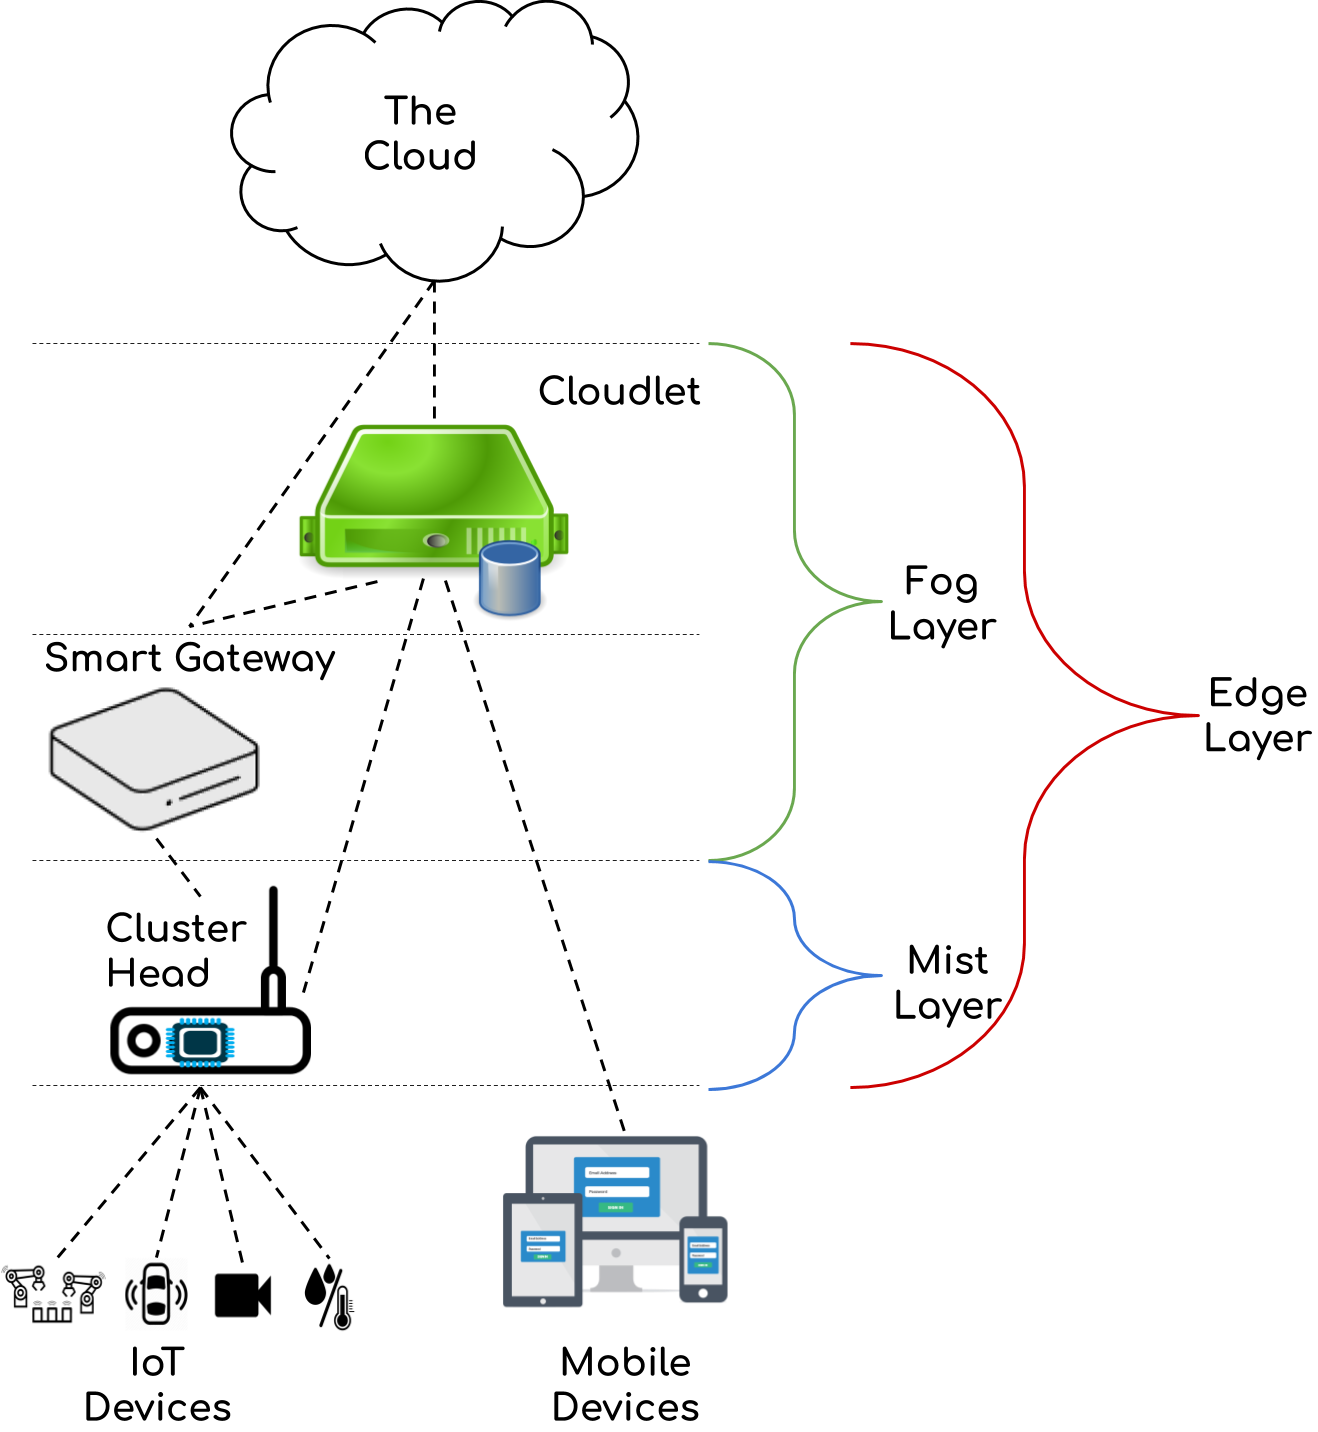
\includegraphics[scale=0.15]{figures/network-topology-3-layer.png}
    \caption{Three tier layer network topology, similar to \cite{nsa2017theNextWaveIoTDefinitions}}
    \label{fig:networkTopology3Layer}
\end{figure}
% Describe figure:
The cloud layer is made up of the 

% More detail
The cloud is the one layer where the authors think the technology stack is set. We expect Linux and Kubernetes, the de-facto standard for cloud orchestration, to be here to stay for the foreseeable future. This implies the same for x86\_64 and ARM, the only CPU architectures being supported by Linux. The Internets communication will remain in IPv4 and increasingly IPv6 for the Internet layer and TCP and UDP for the transport layer.\\ 
Quite the contrary is true for the bottom layer, IoT devices and mobile devices, although for the latter to a lesser extend. Communication in the IoT space is very diverse. Some protocols like 802.11 and Mobile

We expect IoT devices to have different software and different 
This can, but must not, include a control plane
The aim is to find the most promesing solution and 




Promesing solution with deep integration into K8s.


In essence, fog is the standard, and edge is the concept. Fog enables repeatable structure in the edge computing concept, so enterprises can push compute out of centralized systems or clouds for better and more scalable performance.
https://www.cisco.com/c/en/us/solutions/enterprise-networks/edge-computing.html


As it's name implies its aim is to develop an edge solution with Kubernetes support.

The need for smart IoT Gateways or fog computing is well established. They make it possible to 

Their design however is not. 
While the problems at the IoT edge — connectivity, manageability, scalability, reliability, security — are being solved as point solutions by enterprises and ecosystem players, there is a need for a foundational industry-wide standard for managing distributed IoT workloads.





IoT has seen a rapid growth over the last few years. According to IoT Analytics the total number of IoT devices is set to surpass the total number of other connected devices around 2021 \cite{StateofIoT:online}. Further, most IoT devices will be used in WPAN \footnote{Wireless Private Area Networks includes technologies like Zigbee,Z-wave and Bluteooth} and WLAN\footnote{Wireless Local Area Networks includes mainly Wi-Fi}. 
% In contrast to 5G, these technologies don't connect to an access point from an Internet provider but rather require another user operated device to connect to the Internet, a so called "gateway"


But fog computing does not come without its drawbacks. Depending on the protocol edge devices need to be close to their peers and slaves and physically accessible for maintenance. Which also poses a major security risk as they could be accessed by malicious intruders. The software maintenance is another critical aspects. Often IoT and edge devices are not update and patched with critical consequences. The "2016 Dyn cyberattack" used IoT devices like residential gateways, smart fridges, baby phones ect. to bring down the DNS-Servers operated by Dyn making large part of the Internet unaccessible for hours\cite{dynAttack}. The authors also stress that "large number of IoT devices are accessible over public Internet" and that "security (if considered at all) is often an afterthought in the architecture of many wide spread IoT devices"\cite{dynAttack}.\\
The question is then, how can manage and secure those devices. In this thesis, I will solely be concerned with the software aspect, which can mitigate some effects of exposing physical hardware to more accessible places.\\
Many challenges facing edge devices today have already been solved, although in a slight different context: The cloud\cite{IntroducingDejanBosanac:KubernetesIoTEdgeWorkingGroup}. In the cloud 




% Note: Maybe make a graph cloud setup, user connecting to nodes, VS fog computing, sensors and users connecting to gateways and gateway to cloud.  https://www.einfochips.com/blog/iot-gateways-drivers-for-fog-computing/

Kubernetes IoT Edge Working Group is a collaboration between Eclipse IoT Working Group and its 40-member companies, 35 open source projects, and Kubernetes ecosystem. It will define terminology, identify gaps in deployment and management, and educate the market on common use cases.
https://www.dailyhostnews.com/eclipse-foundation-and-cncf-working-together-to-bring-kubernetes-to-iot-edge
}